\graphicspath{{./images/molecules/orbitals/tetra-pyrene/}}
\begin{figure}[h!]
	\centering
\begin{minipage}{\textwidth}\centering
\mybox{
\begin{tabular}{lrccc}
\multicolumn{2}{c}{\textbf{Tetra-Pyrene}} & Model & HOMO & LUMO\\
\multicolumn{2}{c}{\textbf{}}
&\multirow{3}{*}{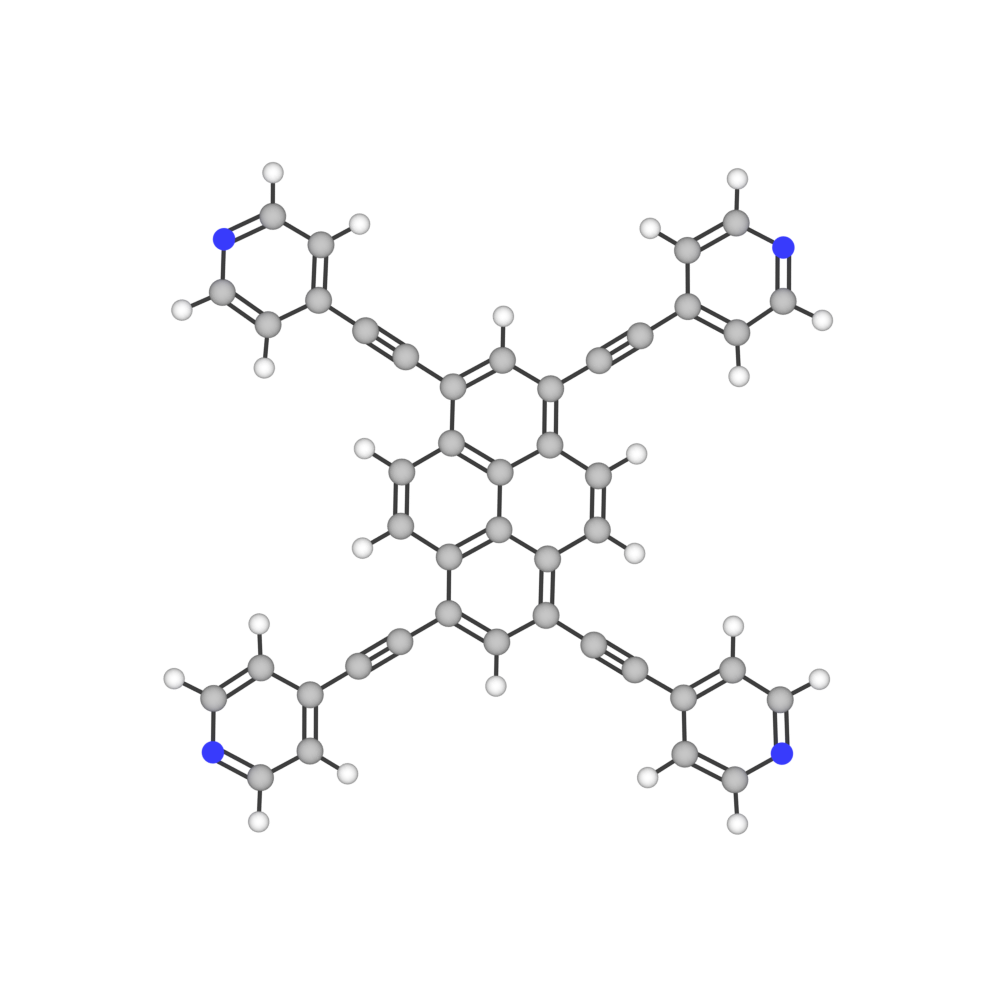
\includegraphics[width=2.7cm]{model}}
&\multirow{3}{*}{
\includegraphics[width=2.7cm]{homo}}
&\multirow{3}{*}{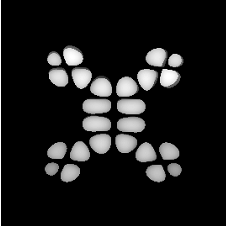
\includegraphics[width=2.7cm]{lumo}}\\
&&&& \\
\# Atoms & &&&\\
\# $e^-$ & 218 &&&\\
\# Orbitals & 109 &&&\\
$E_{Gap}$ &  \SI{}{\electronvolt} &&& \\
&&&& \\
&&& \SI{-11.56190}{\electronvolt} & \SI{-10.18613}{\electronvolt} \\
\end{tabular}
}
\end{minipage}
	\subfigure[]{
		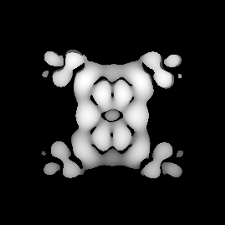
\includegraphics[width=2.7cm]{int-homo-1}
	}
	\subfigure[HOMO - 1]{
		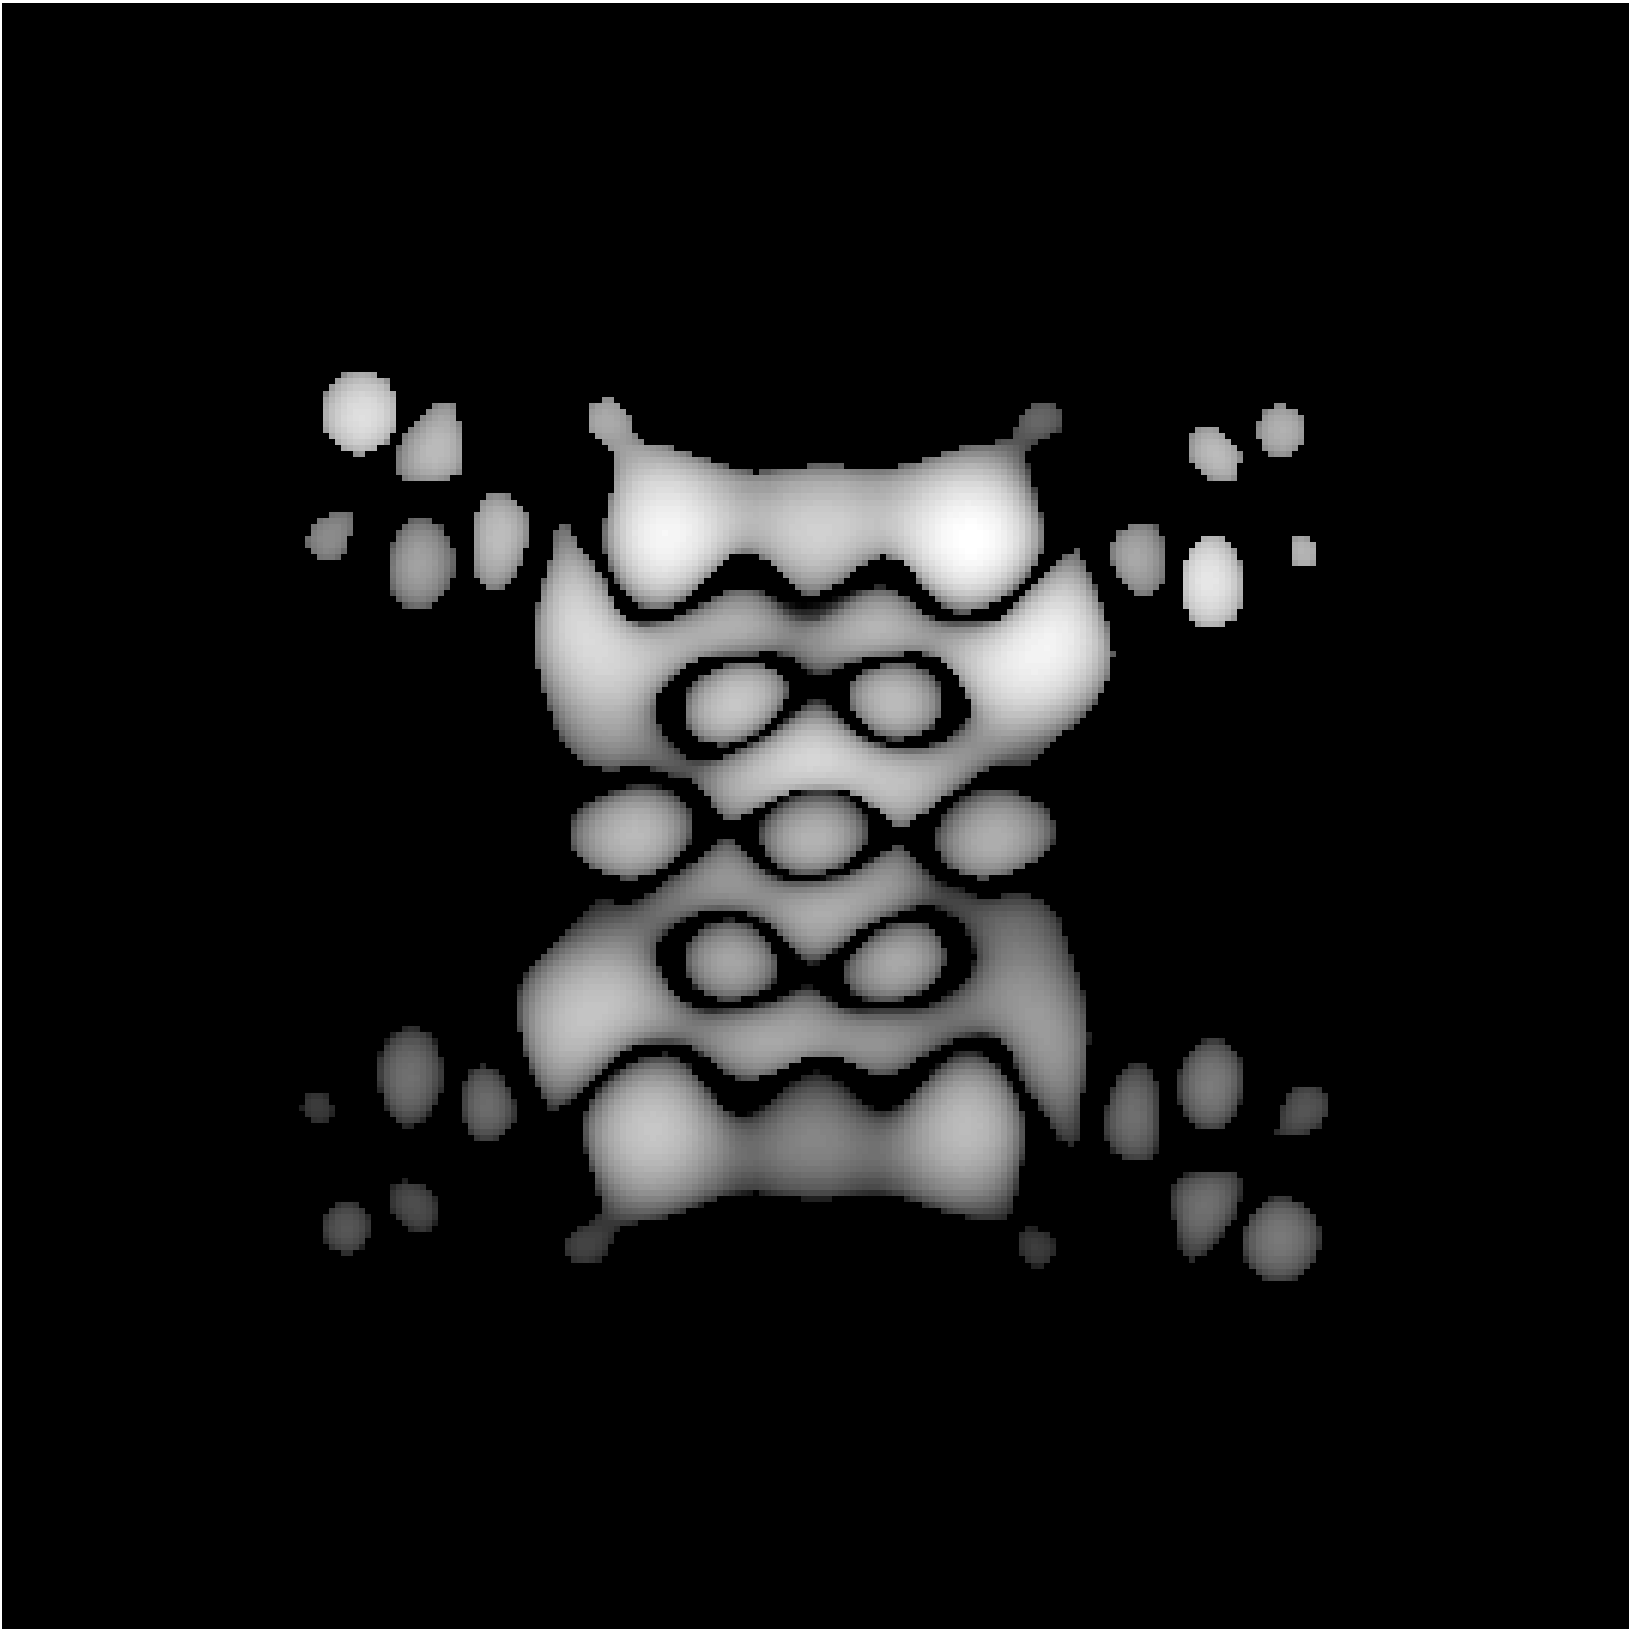
\includegraphics[width=2.7cm]{homo-1}
	}
	\subfigure[LUMO + 1]{
		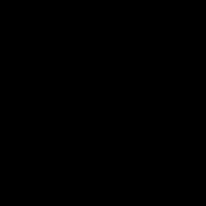
\includegraphics[width=2.7cm]{lumo-1}
	}
	\subfigure[]{
		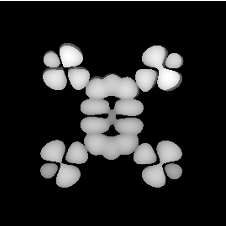
\includegraphics[width=2.7cm]{int-lumo-1}
			
	}
	%%%%%%%%%%%%%%%%%%%%%%%%%%%%%%%%%%%%%%%%%
	\subfigure[]{
		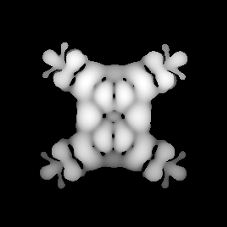
\includegraphics[width=2.7cm]{int-homo-2}
		
	}
	\subfigure[HOMO - 2]{
		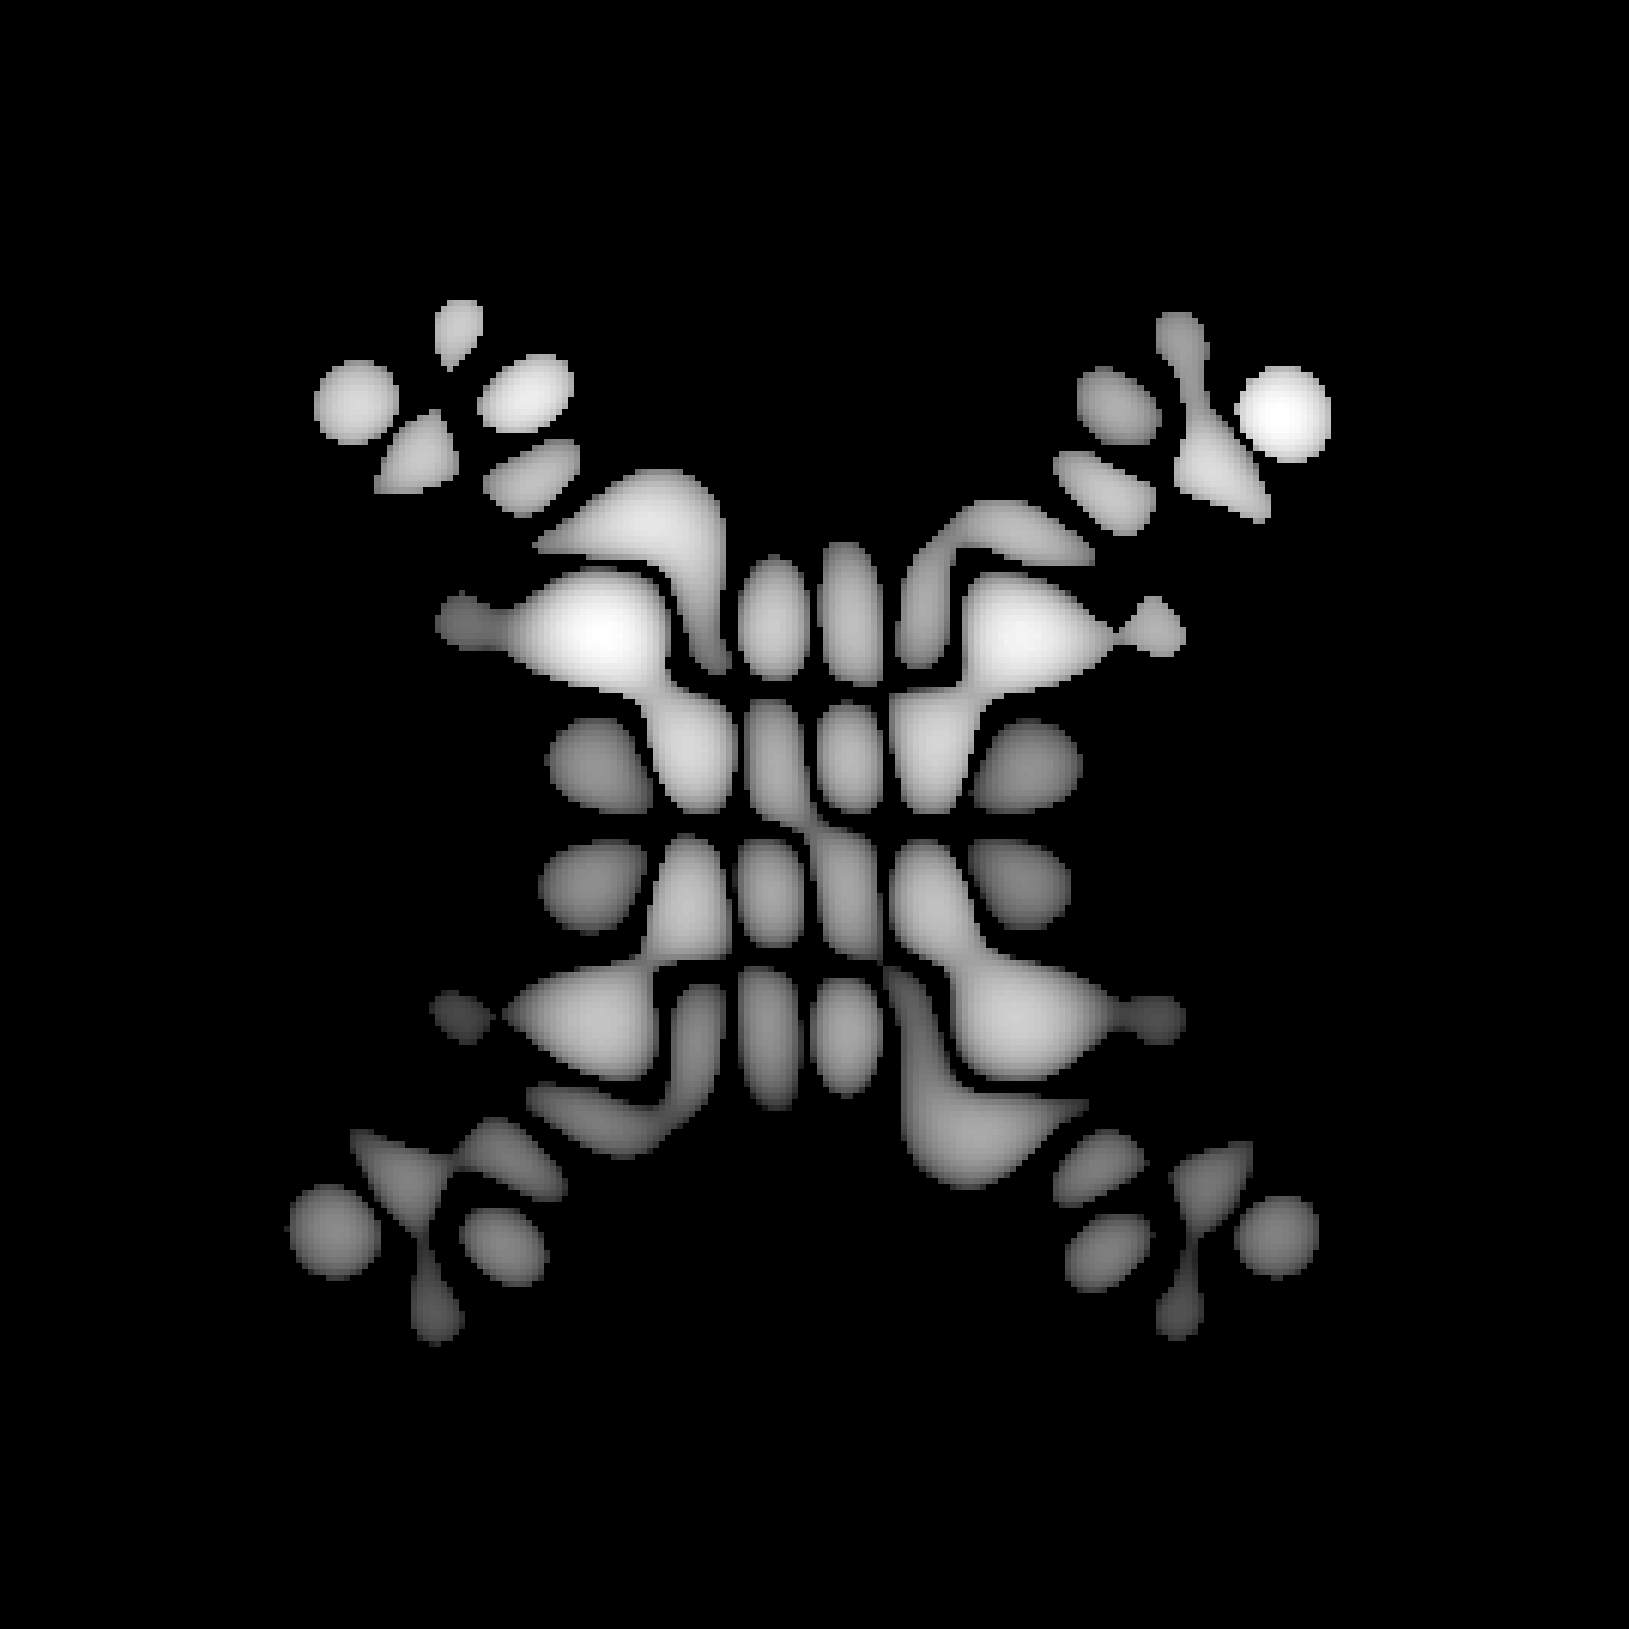
\includegraphics[width=2.7cm]{homo-2}
	}
	\subfigure[LUMO + 2]{
		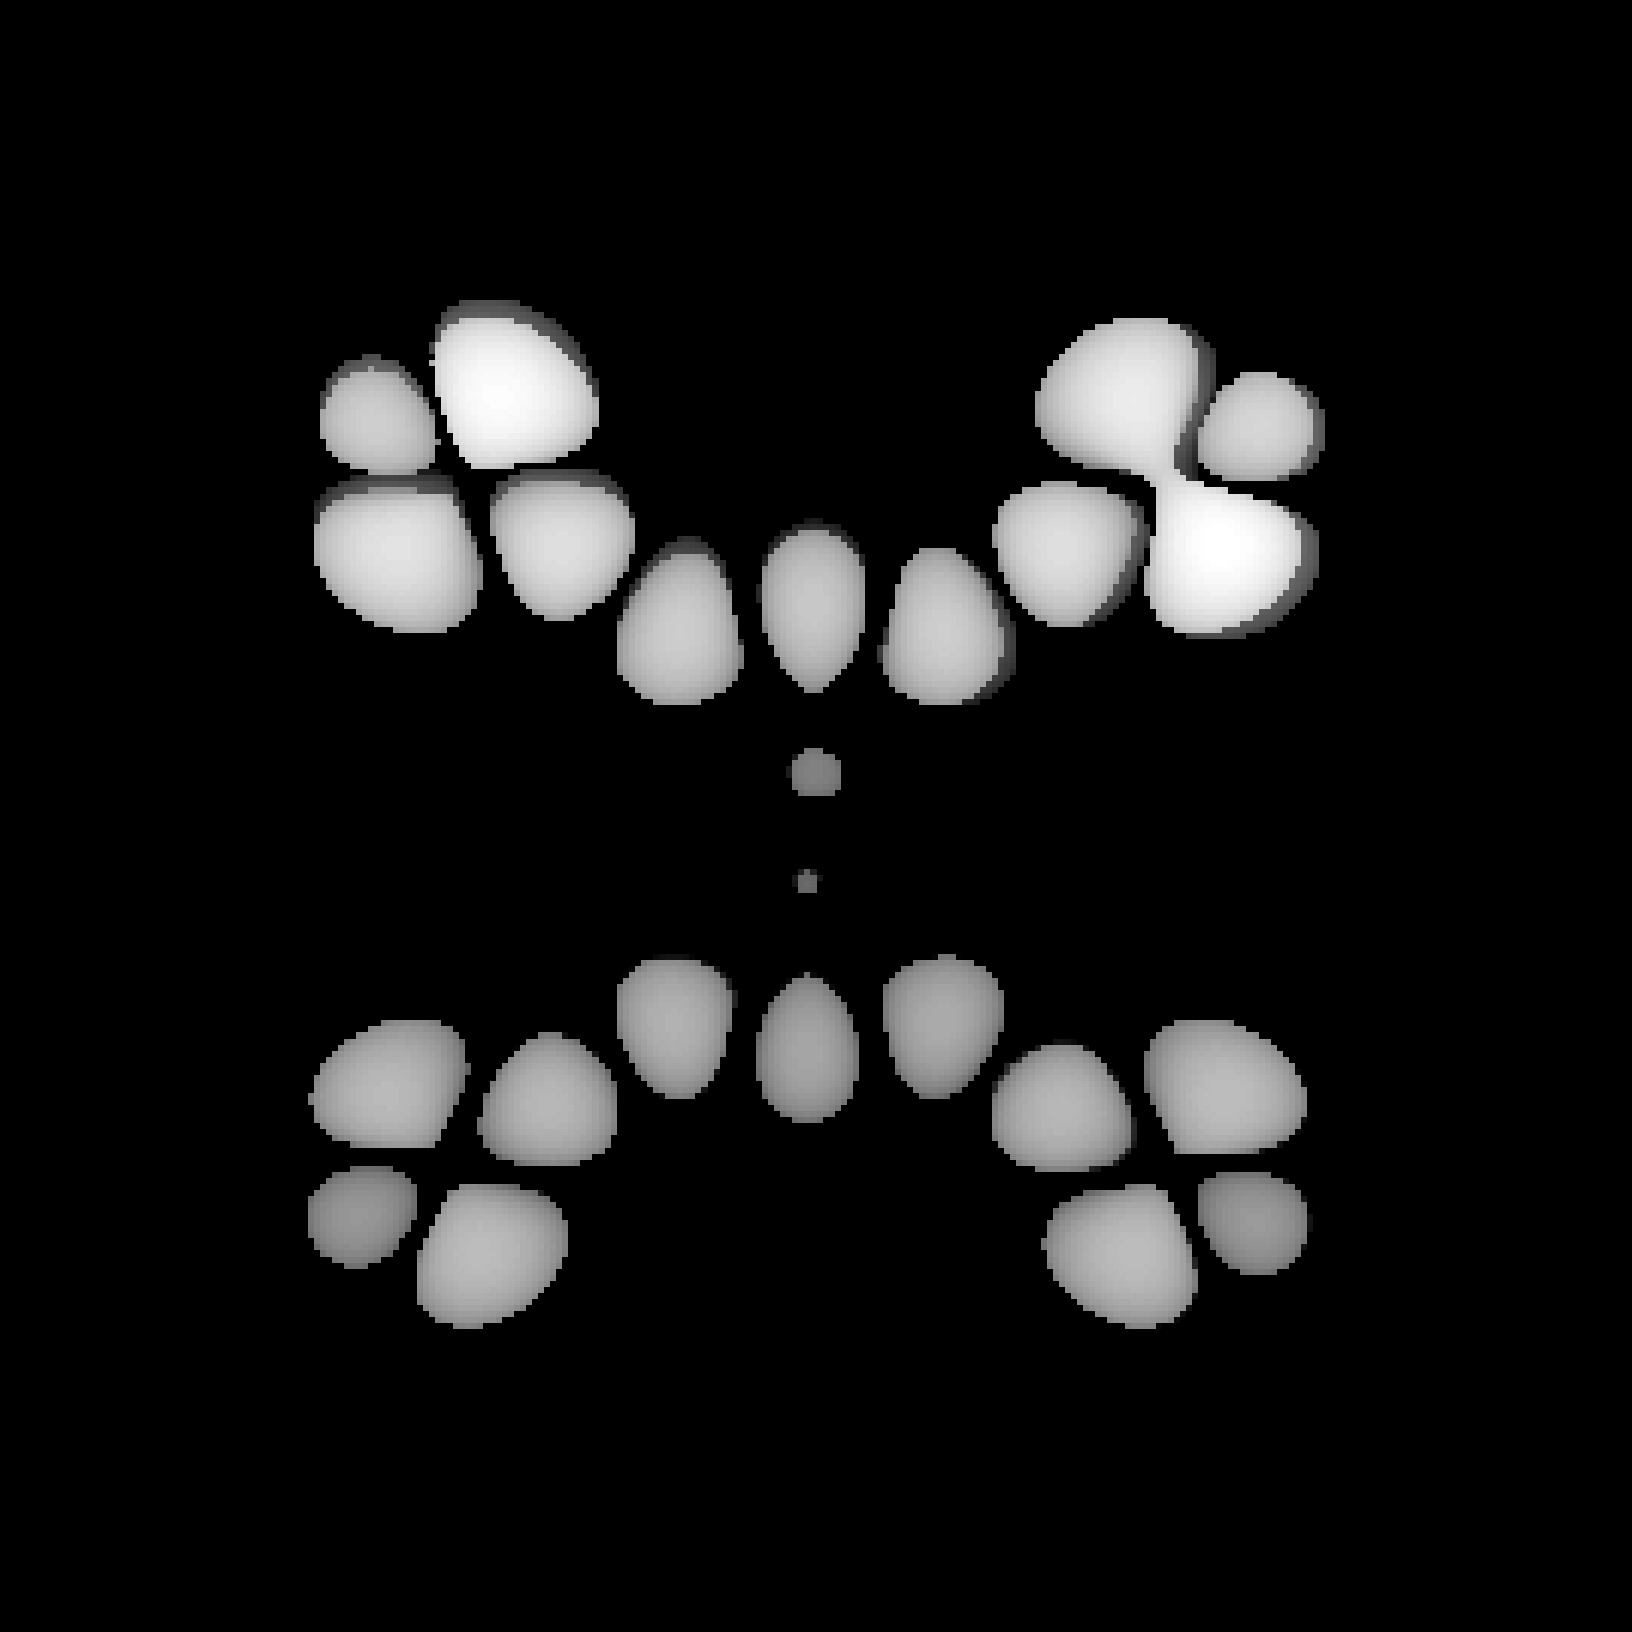
\includegraphics[width=2.7cm]{lumo-2}
	}
	\subfigure[]{
		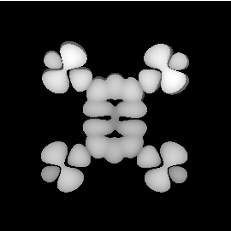
\includegraphics[width=2.7cm]{int-lumo-2}
			
	}
	%%%%%%%%%%%%%%%%%%%%%%%%%%%%%%%%%%%%%%%%%
	\subfigure[]{
		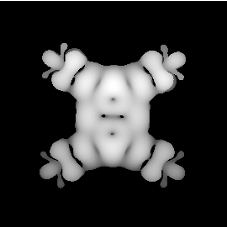
\includegraphics[width=2.7cm]{int-homo-3}
		
	}
	\subfigure[HOMO - 3]{
		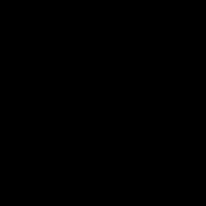
\includegraphics[width=2.7cm]{homo-3}
	}
	\subfigure[LUMO + 3]{
		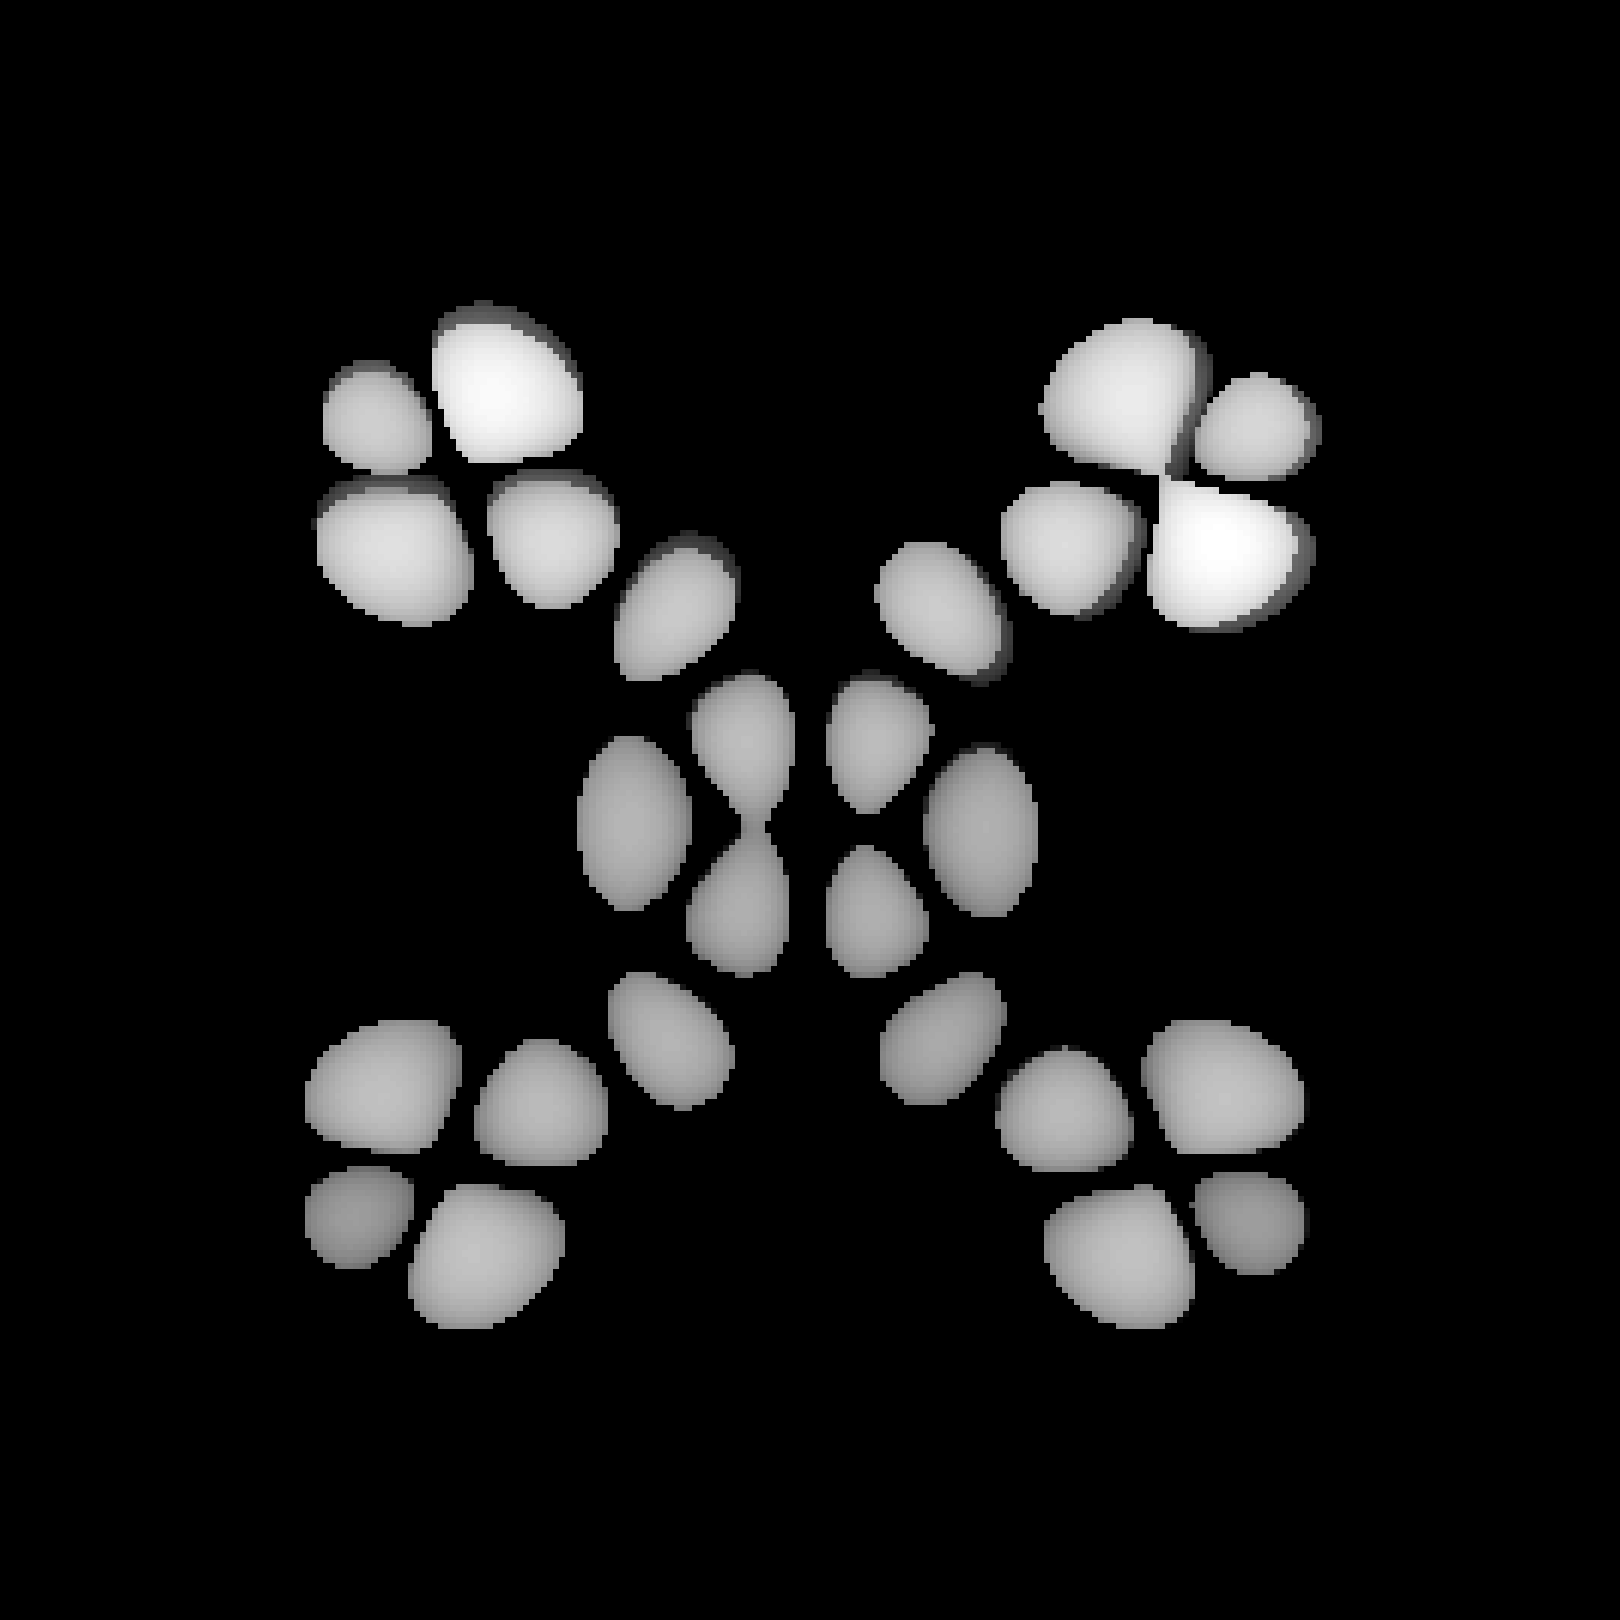
\includegraphics[width=2.7cm]{lumo-3}
	}
	\subfigure[]{
		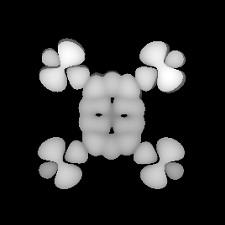
\includegraphics[width=2.7cm]{int-lumo-3}
			
	}
	%%%%%%%%%%%%%%%%%%%%%%%%%%%%%%%%%%%%%%%%%
	\subfigure[]{
		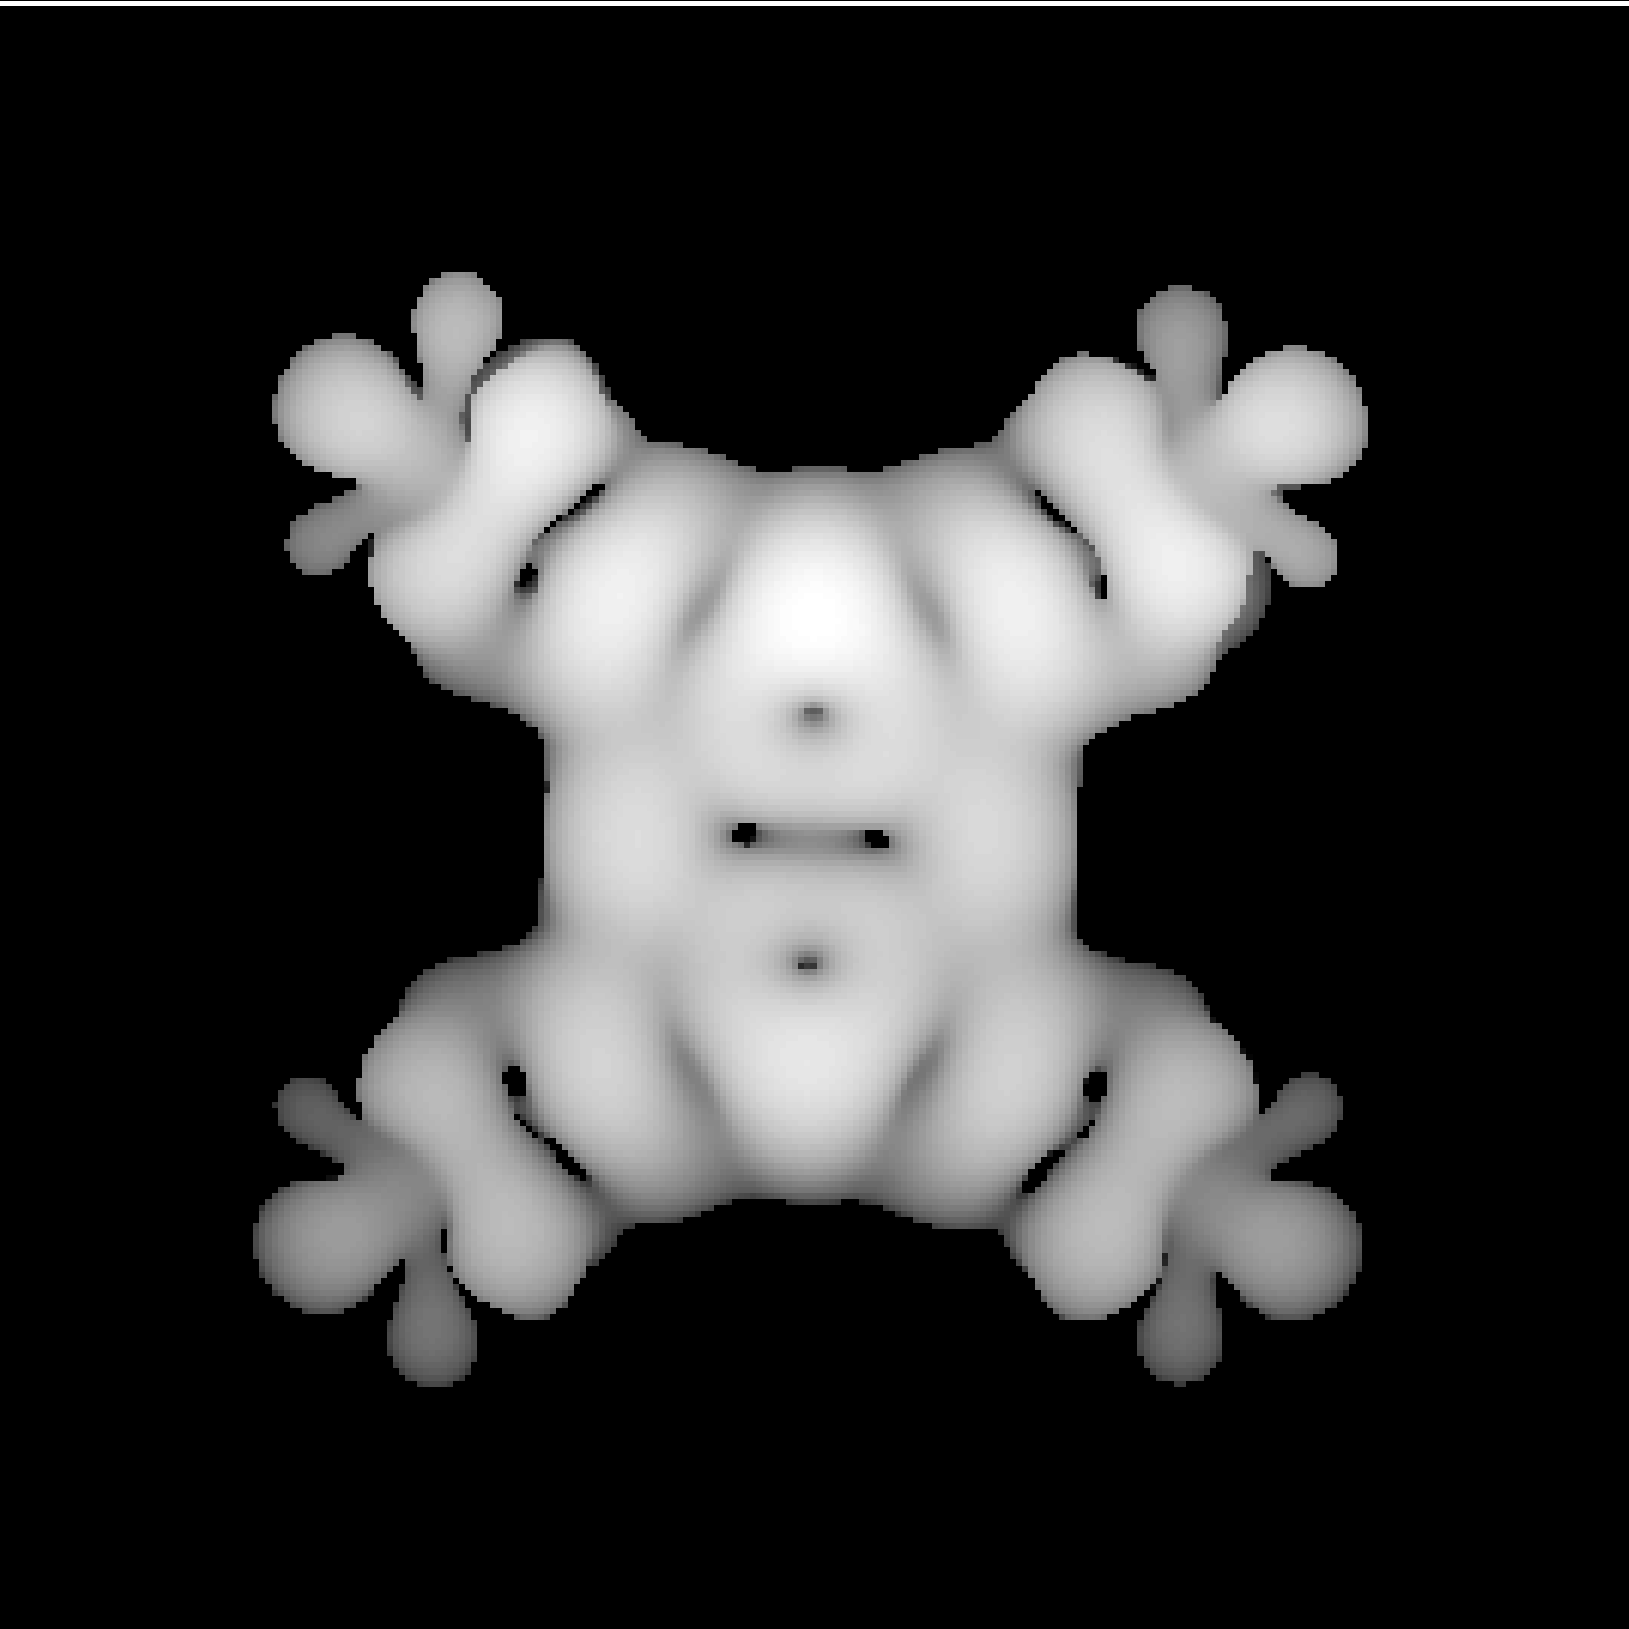
\includegraphics[width=2.7cm]{int-homo-4}
		
	}
	\subfigure[HOMO - 4]{
		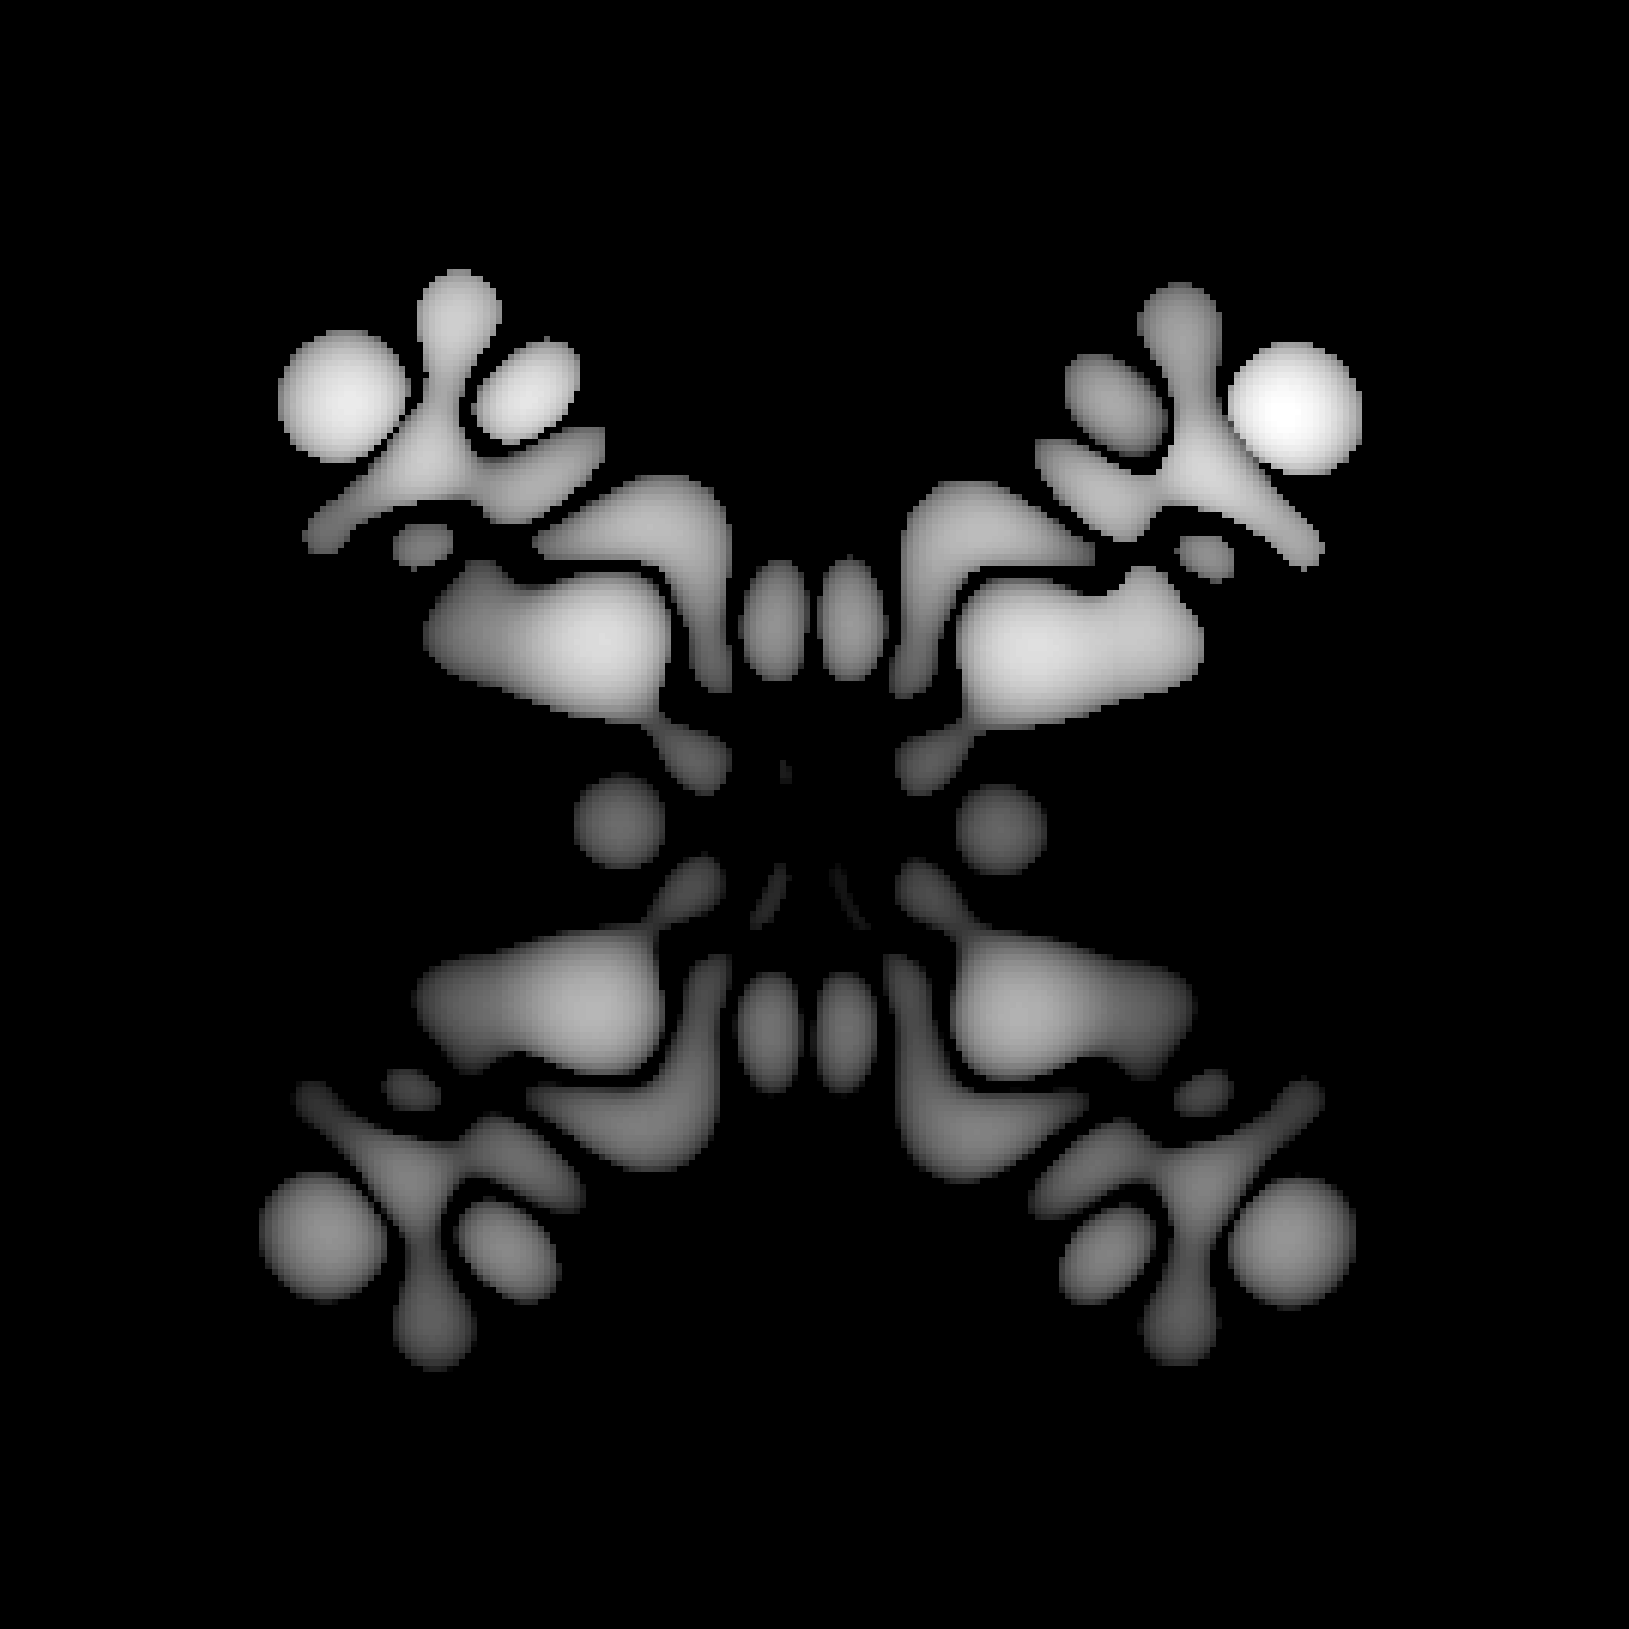
\includegraphics[width=2.7cm]{homo-4}
	}
	\subfigure[LUMO + 4]{
		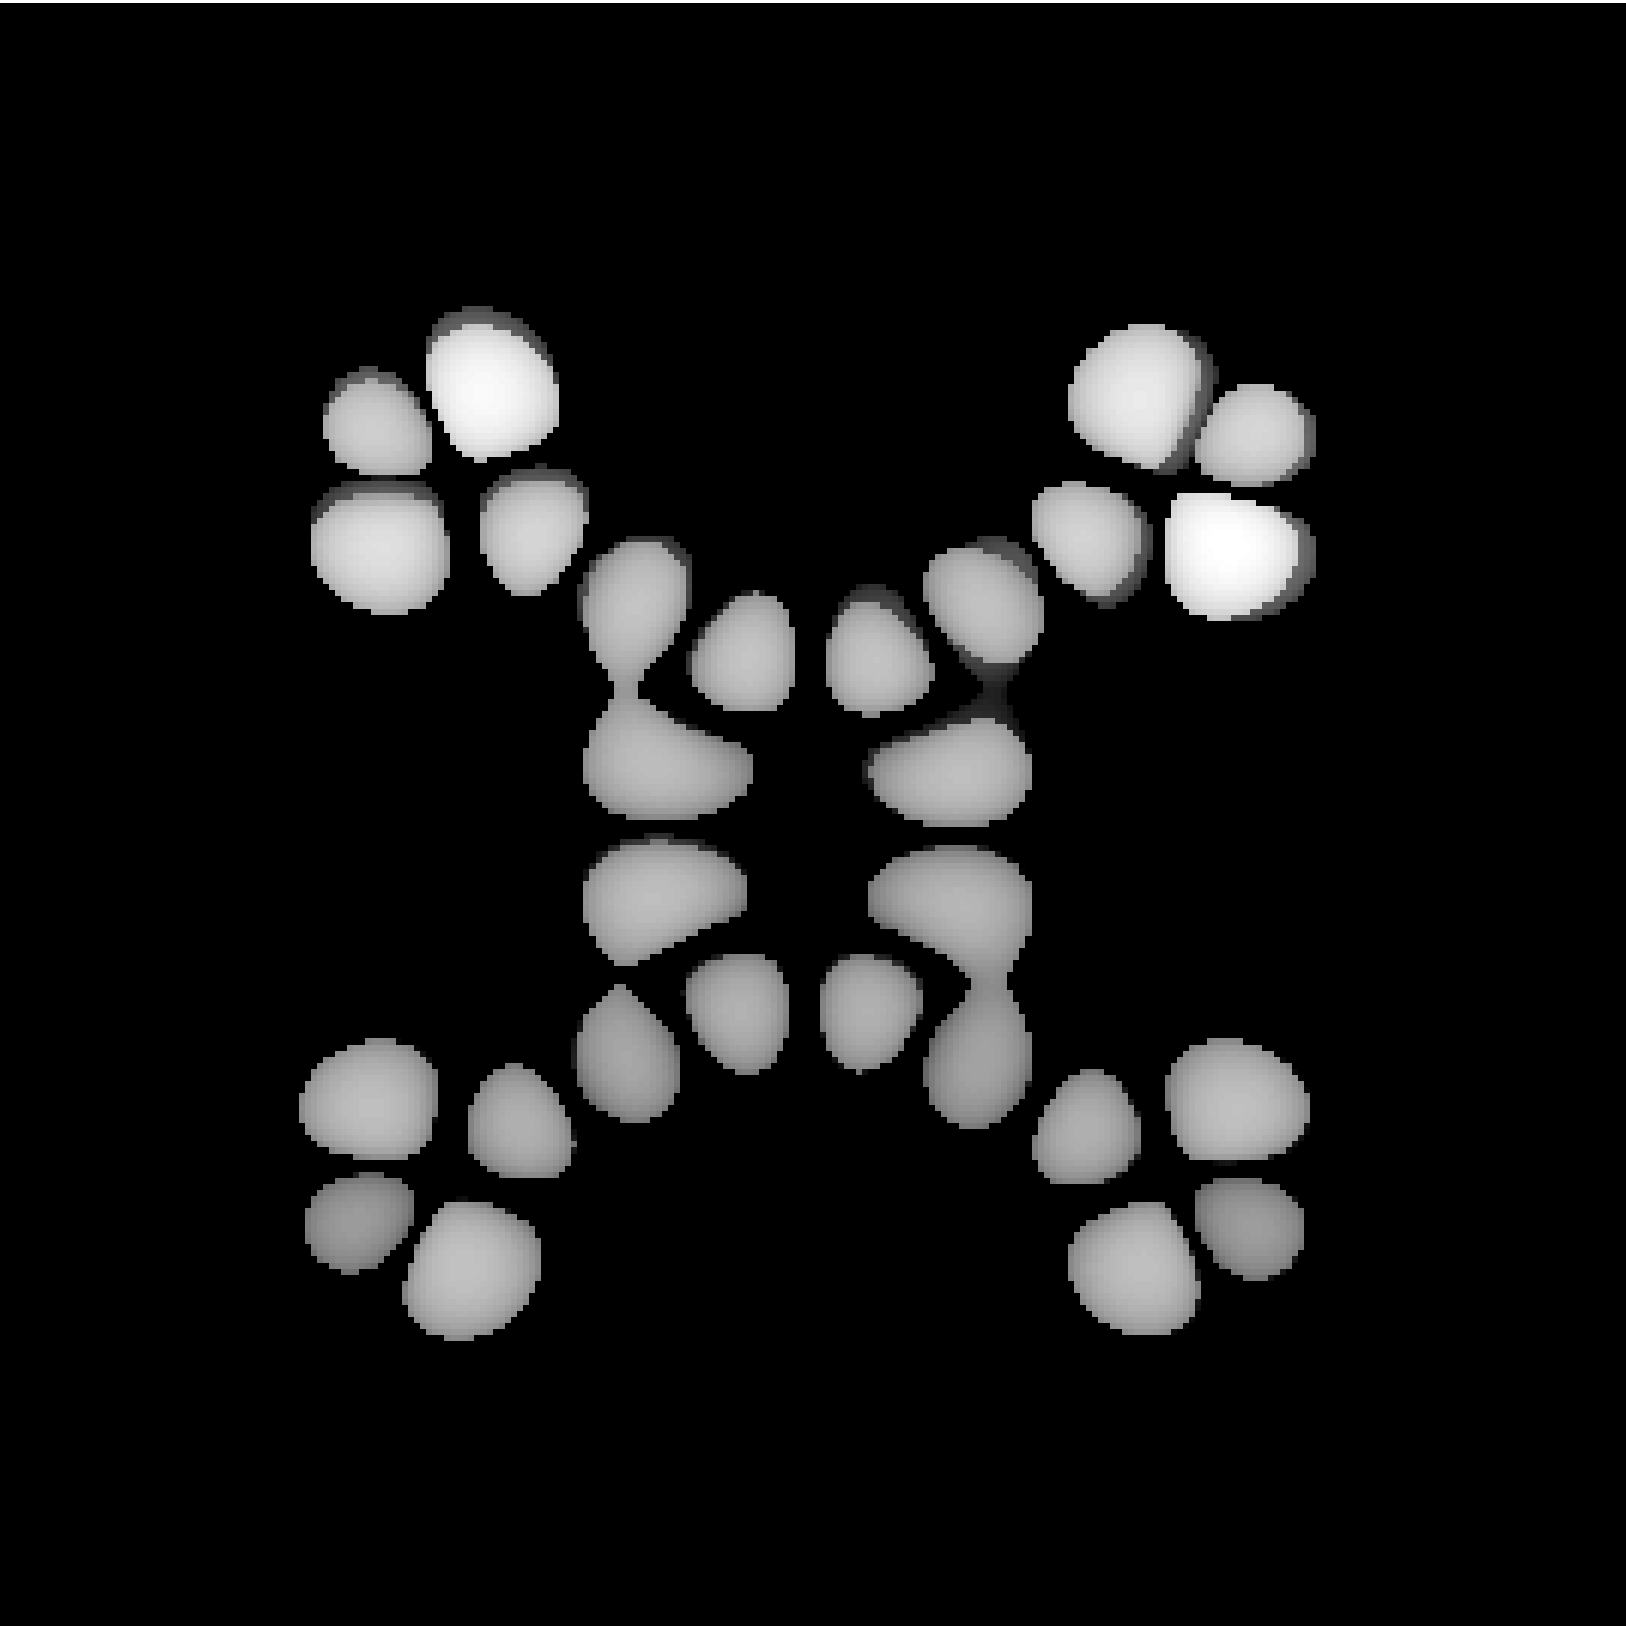
\includegraphics[width=2.7cm]{lumo-4}
	}
	\subfigure[]{
		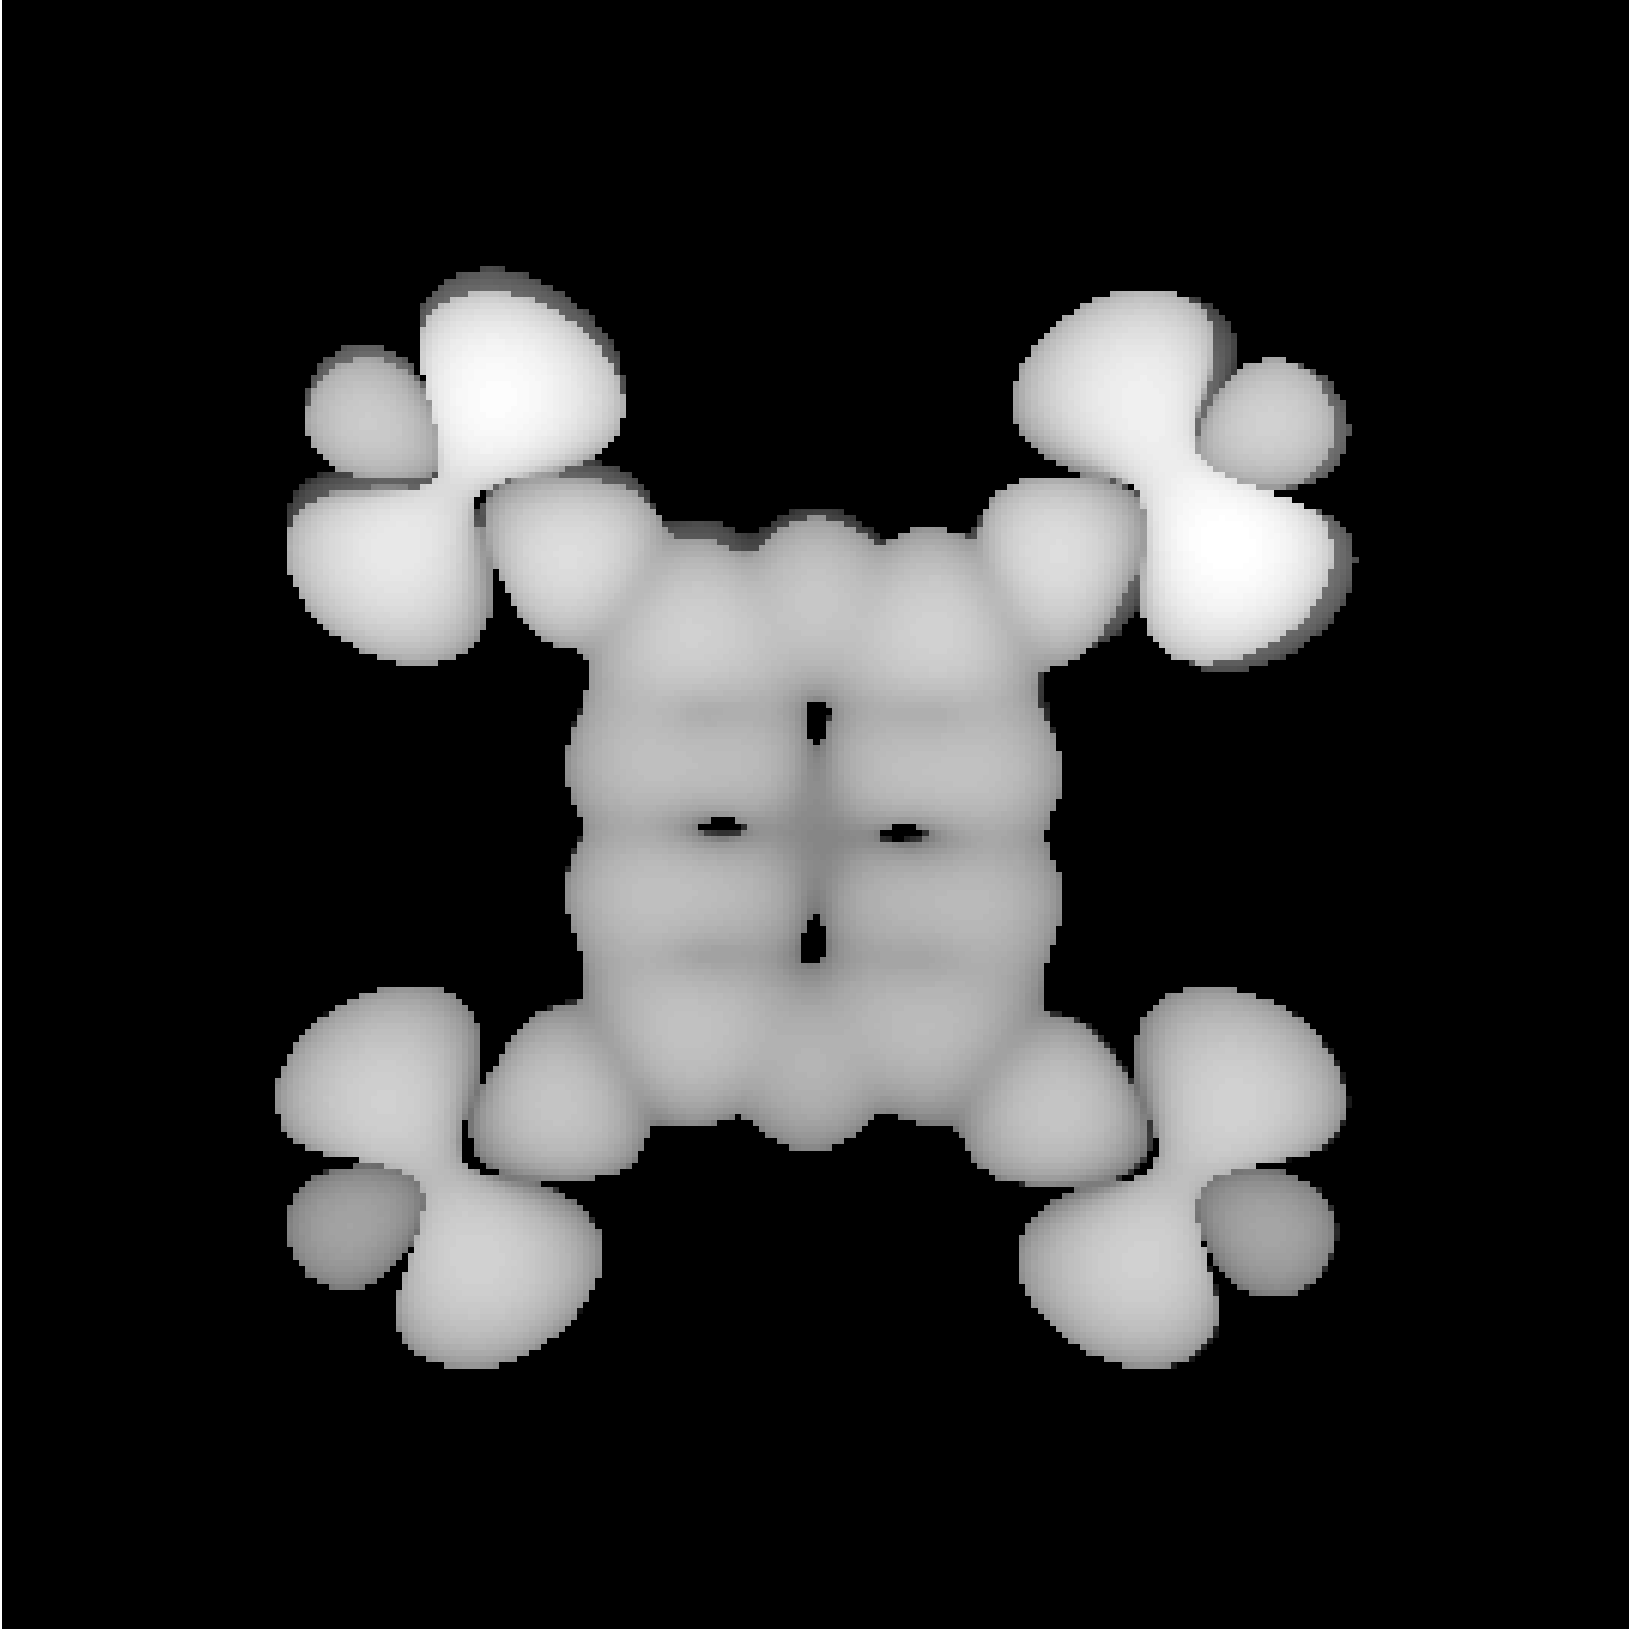
\includegraphics[width=2.7cm]{int-lumo-4}
			
	}
	%%%%%%%%%%%%%%%%%%%%%%%%%%%%%%%%%%%%%%%%%
	\subfigure[]{
		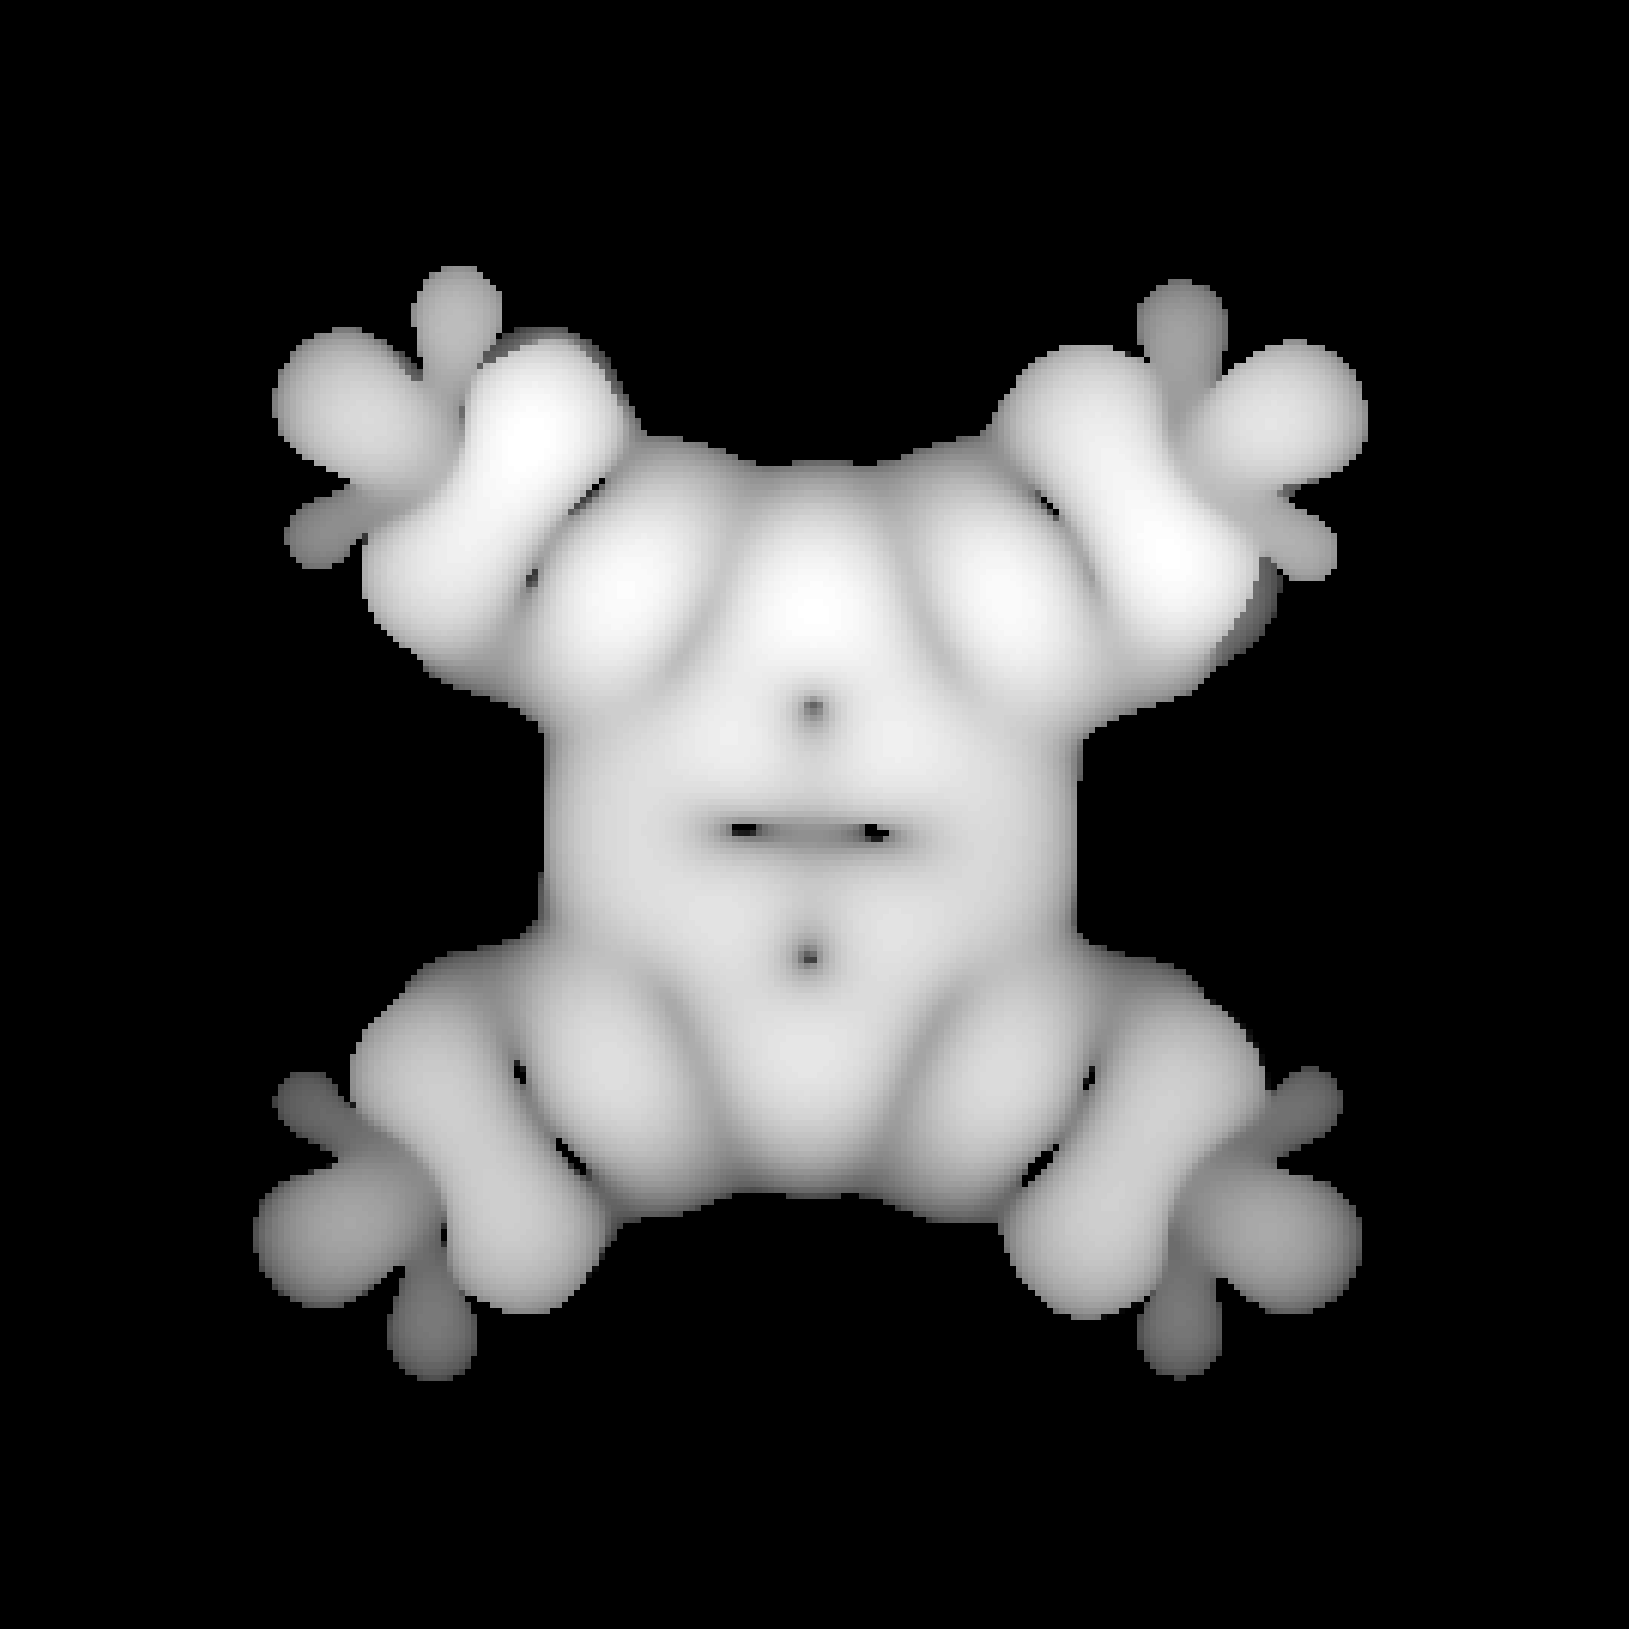
\includegraphics[width=2.7cm]{int-homo-5}
		
	}
	\subfigure[HOMO - 5]{
		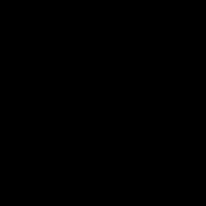
\includegraphics[width=2.7cm]{homo-5}
	}
	\subfigure[LUMO + 5]{
		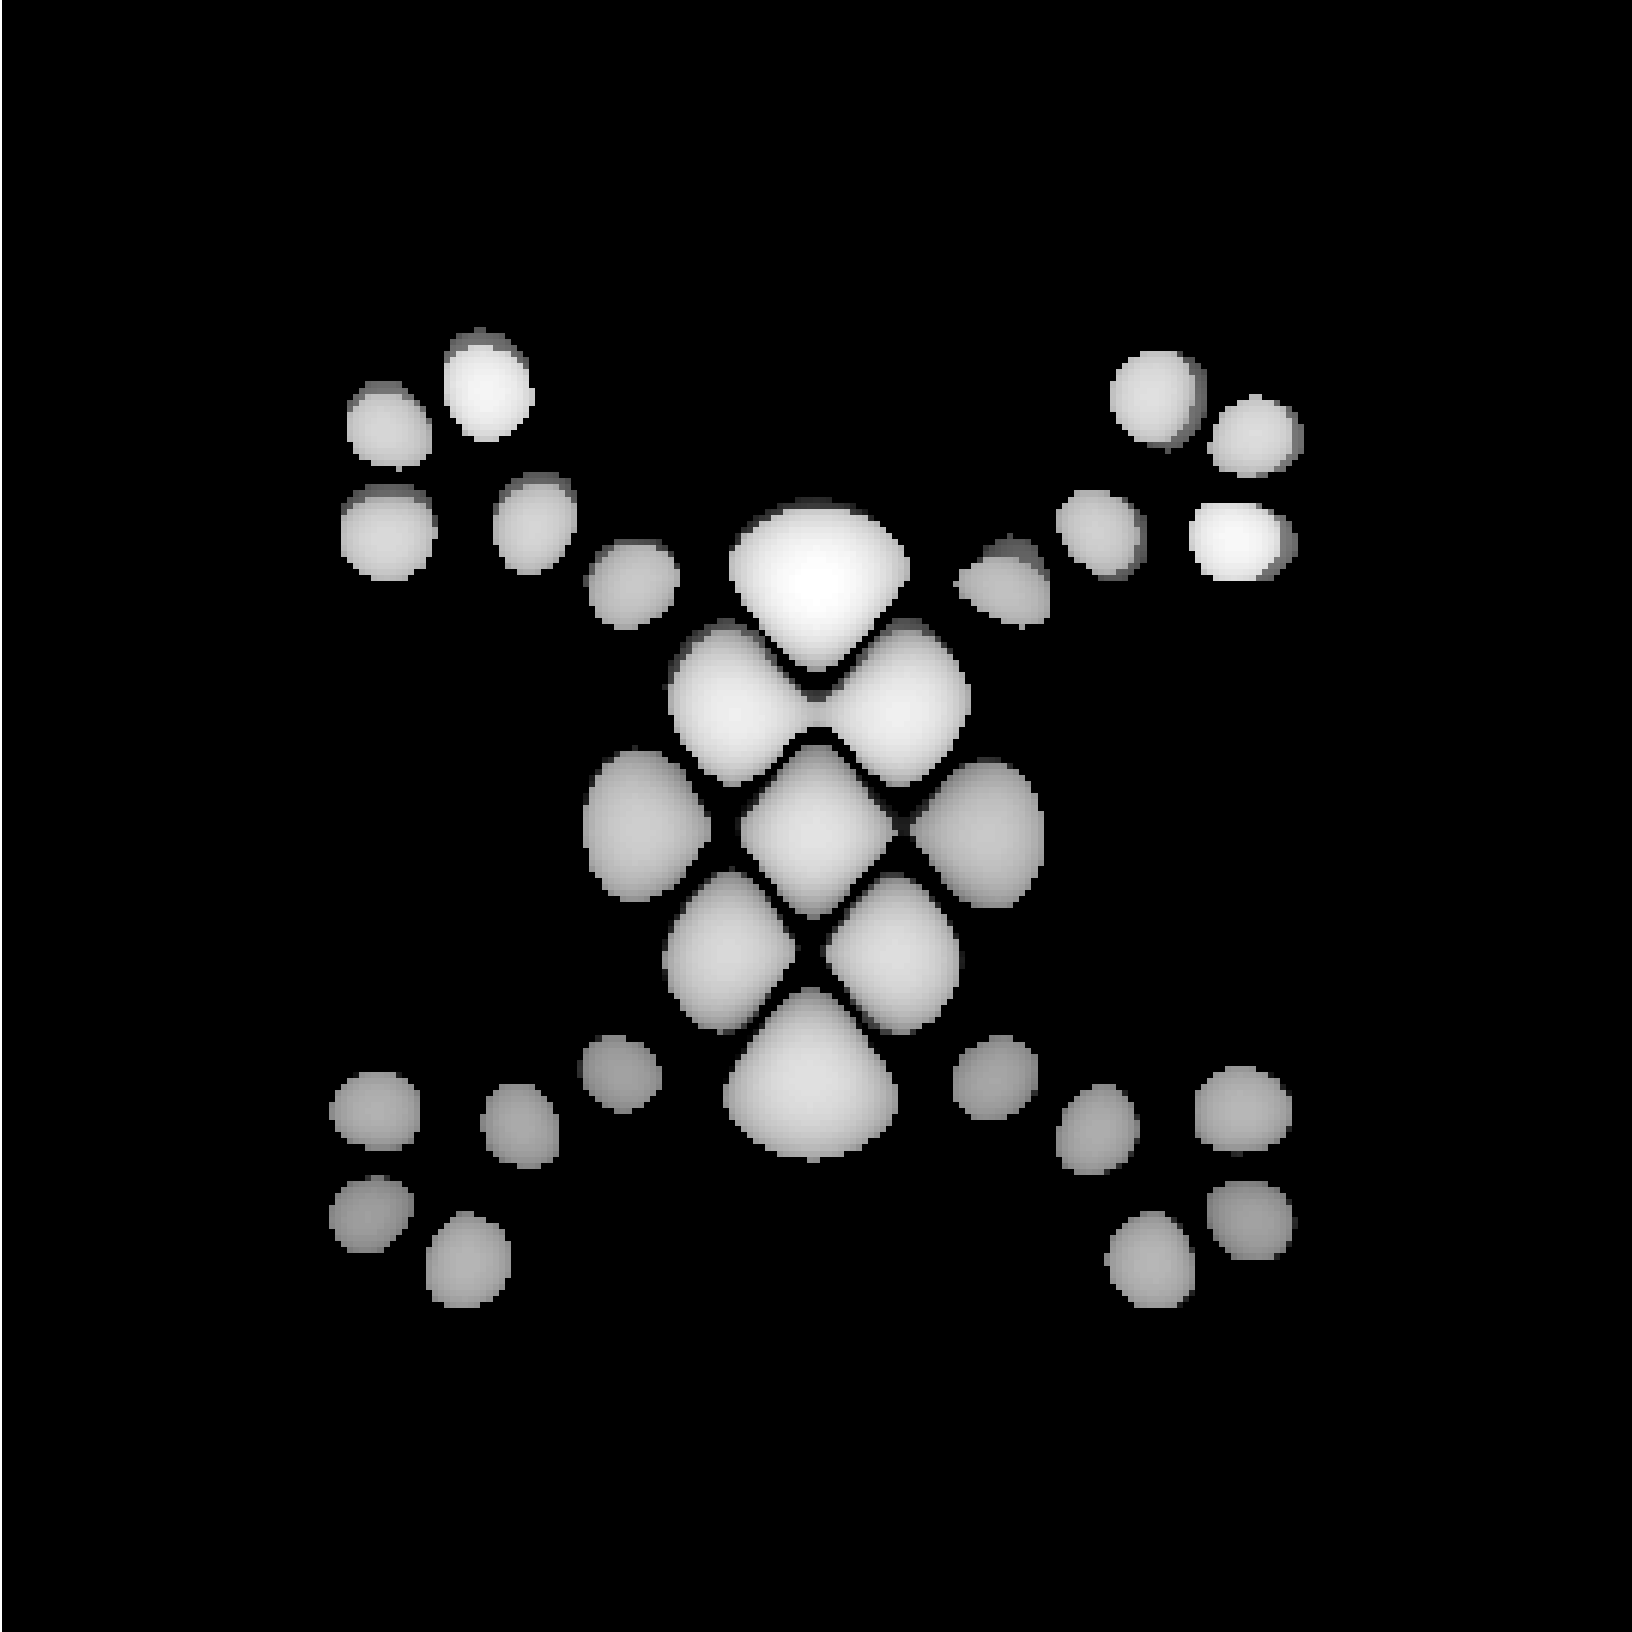
\includegraphics[width=2.7cm]{lumo-5}
	}
	\subfigure[]{
		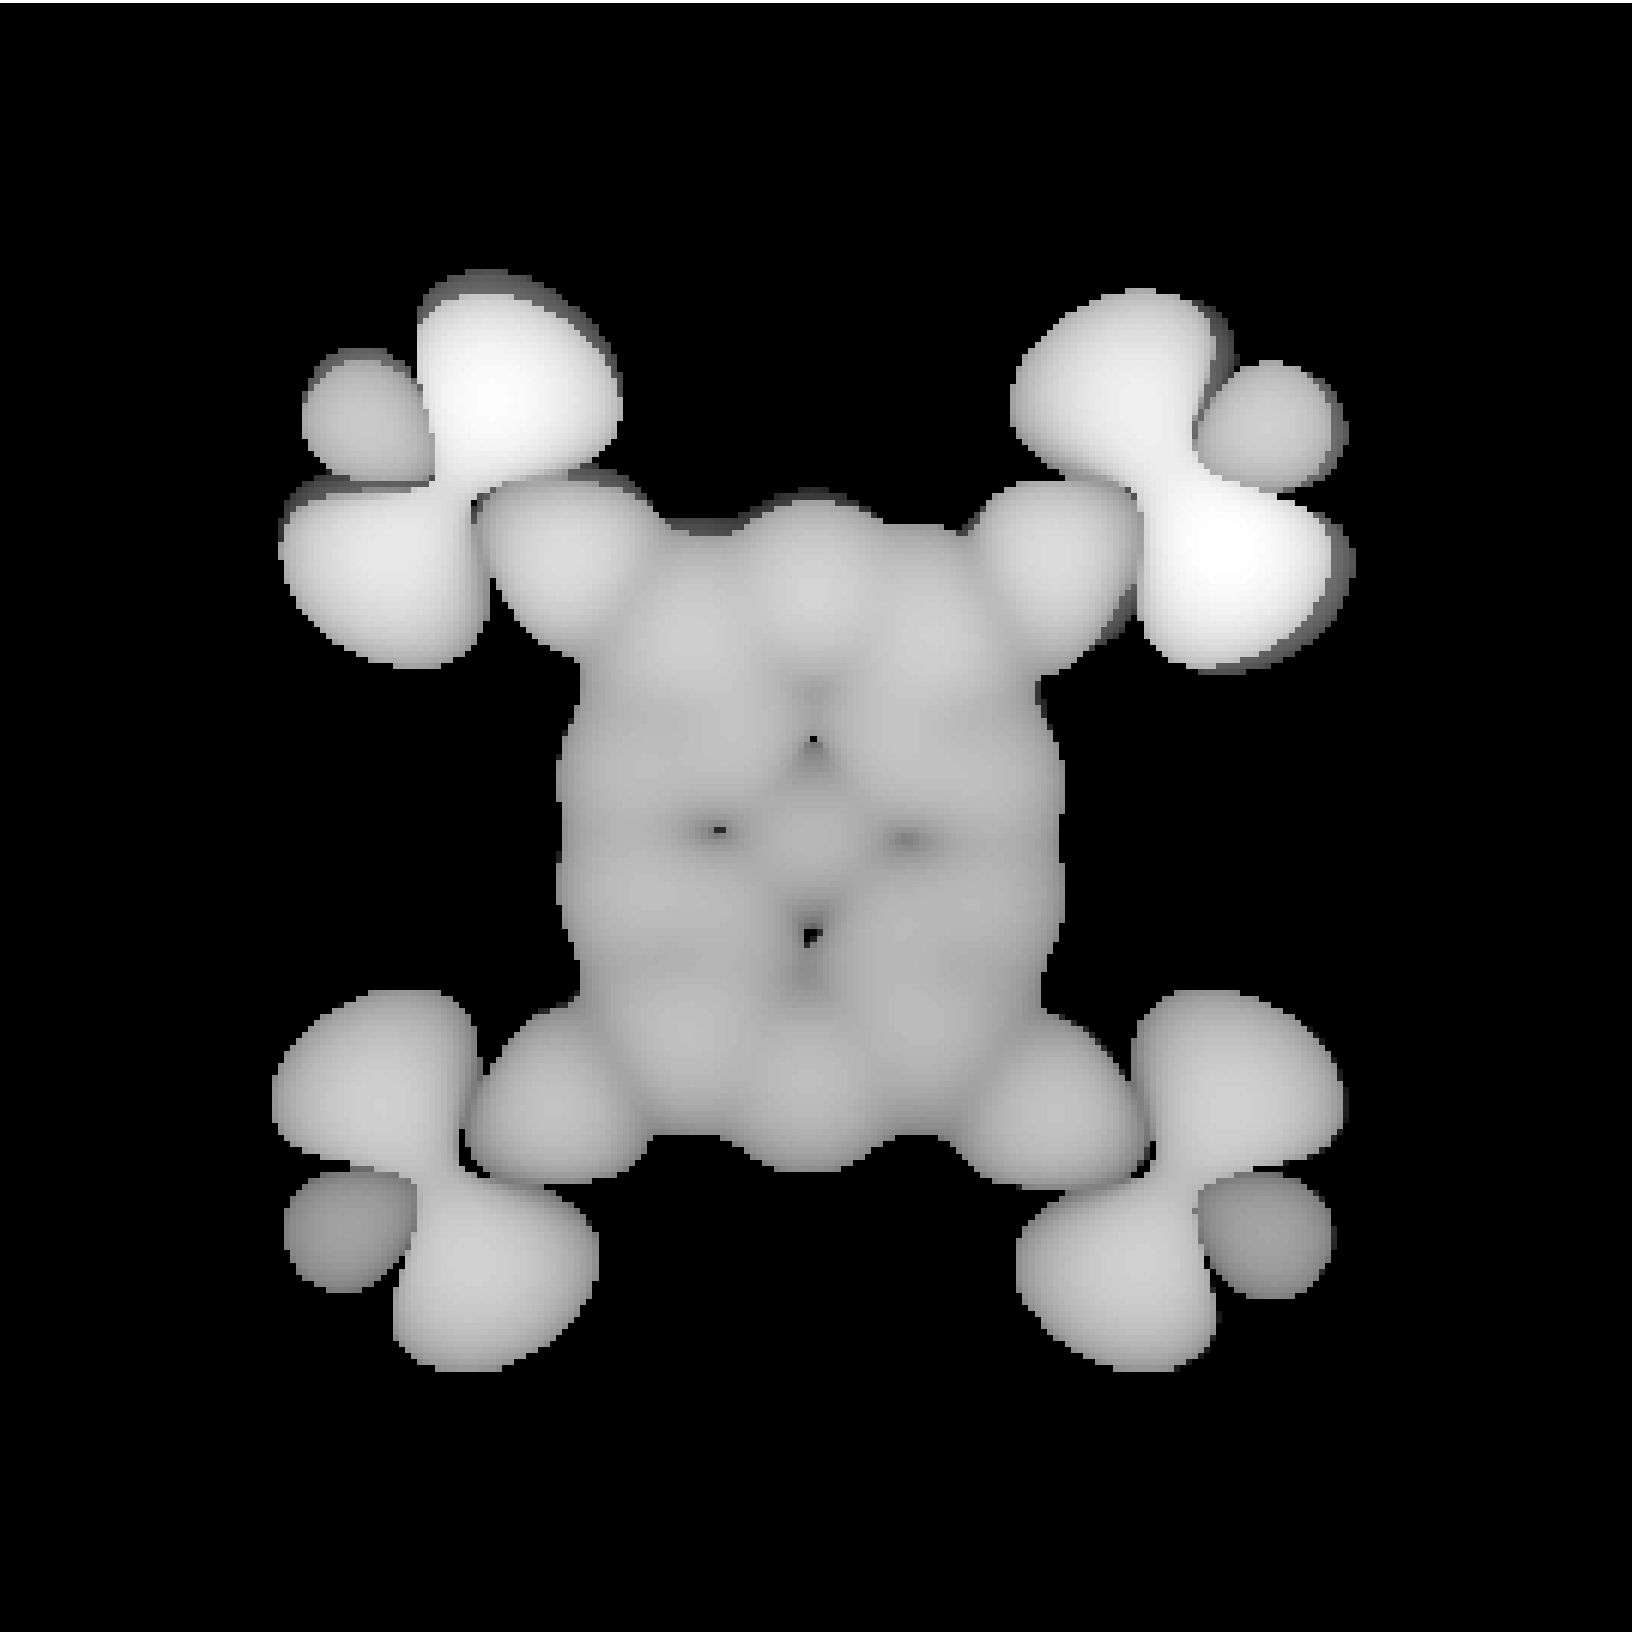
\includegraphics[width=2.7cm]{int-lumo-5}
			
	}
	\caption{EHT calculated molecular orbitals. HOMO and LUMO states together with five neighboring states (shown in the same column). Inner two columns show HOMO \& LUMO states. Outer columns show integration of states as STM image estimation if all states to $E_F$ were contributing equally. Images are \SI{2.5}{\nano \meter} wide}
	
\end{figure}
\vfill